% Don't touch this %%%%%%%%%%%%%%%%%%%%%%%%%%%%%%%%%%%%%%%%%%%
\documentclass[11pt]{article}
\usepackage{fullpage}
\usepackage[left=1in,top=1in,right=1in,bottom=1in,headheight=3ex,headsep=3ex]{geometry}
\usepackage{graphicx}
\usepackage{float}
\renewcommand{\theenumi}{\Alph{enumi})}

\newcommand{\blankline}{\quad\pagebreak[2]}
%%%%%%%%%%%%%%%%%%%%%%%%%%%%%%%%%%%%%%%%%%%%%%%%%%%%%%%%%%%%%%

% Modify Course title, instructor name, semester here %%%%%%%%

\title{\textbf{GGR424: Transportation Geography \& Planning}}
\author{Jeff Allen}
\date{Winter, 2022}

%%%%%%%%%%%%%%%%%%%%%%%%%%%%%%%%%%%%%%%%%%%%%%%%%%%%%%%%%%%%%%

% Don't touch this %%%%%%%%%%%%%%%%%%%%%%%%%%%%%%%%%%%%%%%%%%%
\usepackage[sc]{mathpazo}
\linespread{1.05} % Palatino needs more leading (space between lines)
\usepackage[T1]{fontenc}
\usepackage[mmddyyyy]{datetime}% http://ctan.org/pkg/datetime
\usepackage{advdate}% http://ctan.org/pkg/advdate
\newdateformat{syldate}{\twodigit{\THEMONTH}/\twodigit{\THEDAY}}
\newsavebox{\MONDAY}\savebox{\MONDAY}{Mon}% Mon
\newcommand{\week}[1]{%
	%  \cleardate{mydate}% Clear date
	% \newdate{mydate}{\the\day}{\the\month}{\the\year}% Store date
	\paragraph*{\kern-2ex\quad #1, \syldate{\today} - \AdvanceDate[4]\syldate{\today}:}% Set heading  \quad #1
	%  \setbox1=\hbox{\shortdayofweekname{\getdateday{mydate}}{\getdatemonth{mydate}}{\getdateyear{mydate}}}%
	\ifdim\wd1=\wd\MONDAY
	\AdvanceDate[7]
	\else
	\AdvanceDate[7]
	\fi%
}
\usepackage{setspace}
\usepackage{multicol}
%\usepackage{indentfirst}
\usepackage{fancyhdr,lastpage}
\usepackage{url}
\pagestyle{fancy}
\usepackage{hyperref}
\usepackage{lastpage}
\usepackage{amsmath}
\usepackage{layout}

\lhead{}
\chead{}
%%%%%%%%%%%%%%%%%%%%%%%%%%%%%%%%%%%%%%%%%%%%%%%%%%%%%%%%%%%%%%

% Modify header here %%%%%%%%%%%%%%%%%%%%%%%%%%%%%%%%%%%%%%%%%
\rhead{\footnotesize Transportation Data Analysis | GGR424}
\lhead{\footnotesize Jeff Allen}
%%%%%%%%%%%%%%%%%%%%%%%%%%%%%%%%%%%%%%%%%%%%%%%%%%%%%%%%%%%%%%
% Don't touch this %%%%%%%%%%%%%%%%%%%%%%%%%%%%%%%%%%%%%%%%%%%
\lfoot{}
\cfoot{\small \thepage/\pageref*{LastPage}}
\rfoot{}

\usepackage{array, xcolor}
\usepackage{color,hyperref}
\definecolor{clemsonorange}{HTML}{f00000}
\hypersetup{colorlinks,breaklinks,linkcolor=clemsonorange,urlcolor=clemsonorange,anchorcolor=clemsonorange,citecolor=black}

\setlength{\parindent}{0em}
\setlength{\parskip}{0.8em}

\usepackage{colortbl}
\usepackage{tabularx,ragged2e}
\usepackage{sectsty}


\usepackage{helvet}

\begin{document}
	\allsectionsfont{\sffamily}
	
	\section*{Transportation Data Analysis Assignment} 
		
	\textit{Due March 3 at 11:59pm}
	
	\vspace{3mm}
	
	This assignment consists of analyzing, mapping, and interpreting various datasets that are commonly used in transportation planning and geography. 
	
	Each part of this assignment focuses on a specific task or research question, and includes creating one or two maps as well as short answer questions.
	
	
	
	
	
	
	\subsection*{General Guidelines}

	
	All the technical questions can be completed using Excel and/or standard GIS software (QGIS or ArcGIS). But you are free to use any other software/tools that you want for any part of this assignment (e.g. R, Python, etc.).
	
	\texttt{data.zip} contains all the data required to complete this assignment.
	
	Please submit your assignment as \textbf{one} pdf or Word doc on Quercus before the due date. Do not upload separate maps or images. Put your name and student number in the header of your assignment.
	
	All maps should be 6.5 inches wide (and thus fit nicely on an 8.5x11 page with 1 inch margins). Please present all maps in a projection that preserves local directions and shapes (e.g. Web Mercator, UTM Zone 17N, etc.). Rotate all maps of Toronto so that Steeles Ave is parallel to the top border of the map (about 17 degrees).
	
	Grading for the maps will be based both on showing the correct data as well as the overall design of the maps (i.e. do they clearly convey the data shown)
	
			
			
	
	
	
	\subsection*{Part 1: Thinking About Accessibility} 
	
	\vspace{-2mm}
	\textbf{\textit{3 marks}}
	
	Consider a city with 10 neighbourhoods, each with 1,000 jobs, that are connected with a single transit line. Assume that the travel time between each adjacent stop is \textbf{10 minutes} and that the headway is \textbf{2 minutes}. 
	
	\begin{figure}[h]
		\centering
		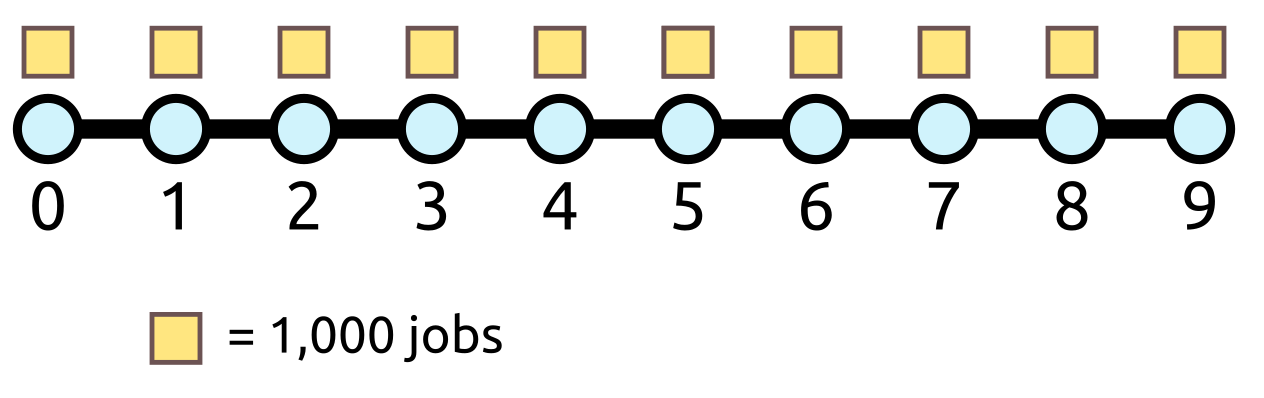
\includegraphics[width=0.5\linewidth]{images/city_plain.png}
	\end{figure}

	The city has grown recently, use your student number to distribute where employment growth is located in the city. Do this by allocating 1,000 additional jobs to each neighbourhood for each digit in your student number.
	
	For example, if your student number is 2013455888, then the distribution of jobs in the city would be as follows:
	
	\begin{figure}[h]
		\centering
		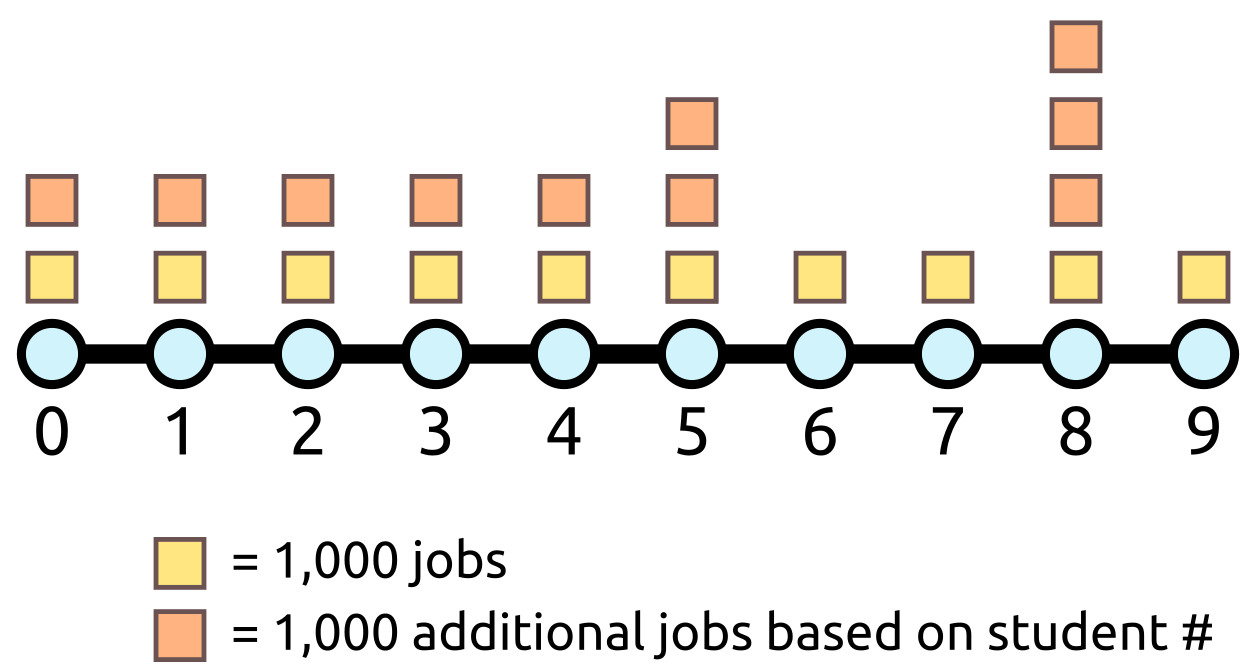
\includegraphics[width=0.5\linewidth]{images/city_jobs.png}
	\end{figure}
	
	
	Answer the following questions based on your student number:
	
	\begin{enumerate}
		
		
		\item If you live in neighbourhood \textbf{0}, how many jobs can you reach in less than or equal to a \textbf{45} minute transit trip? (1) 
		
		\item Using this travel time threshold (\textbf{45} minutes), which neighbourhood(s) has the greatest level of accessibility to jobs? (1) 
		
		\item The city is planning to build a high speed express route to directly connect the stops in neighbourhood \textbf{0} and neighbourhood \textbf{9} in only \textbf{30} minutes (it will also have a headway of \textbf{2} minutes). If you still live in neighbourhood \textbf{0}, how many jobs will you then be able to access in a \textbf{45} minute trip? (1) 
		
	\end{enumerate}

	
	
	
	
	
	
	\subsection*{Part 2: Cycling in Toronto}
	
	\vspace{-2mm}
	\textbf{\textit{7 marks}}
	
	Your task is to map and analyze how and where cycling infrastructure is related to cycling mode share in Toronto. 

	For the infrastructure part, I have prepared data on Bikeshare stations and cycling routes. Data on commuting to work from the 2016 census is in the \texttt{data.zip/census-data-2016} folder.

	\begin{enumerate}
			
		\item Create a map with cycling routes and Bikeshare stations overlaid on top of a choropleth map of cycling mode share for journey to work trips. (3)
		
		\item Describe in a few sentences the patterns between the layers. Is there a strong correlation between cycling infrastructure and mode share? How does this vary in different parts of the city? (1.5)
		
		\item The cycling route data I provided is pretty limited and disconnected. If you wanted to build a more comprehensive cycling network dataset that could be used for network analysis and measuring accessibility, what other routes and attributes (e.g. costs/weights) would you include?  Briefly describe at least three (1.5)
				
		\item Briefly describe one limitation of this census data in examining cycling mode share (0.5)
		
		\item Other than Bikeshare stations, find another \textbf{point} GIS dataset representing some aspect of the built environment that you think would impact cycling travel behaviour. You do not have to create a map, just briefly describe it and provide a link. (0.5)
		
	\end{enumerate}
	
	
	
	
	
	
	\subsection*{Part 3: Pedestrian Accessibility To Libraries} 
	
	\vspace{-2mm}
	\textbf{\textit{6 marks}}
	
	Your task is to map pedestrian accessibility to public libraries. 
	
	In the \texttt{data.zip/part3} folder, there is a pedestrian network dataset pulled from OpenStreetMap. There is also a point file of the locations of public libraries.
	
	
	\begin{enumerate}
		\item Create a map showing walking access isochrones to public libraries in Toronto. Have the map show 2 bands of access one at 750m and another for 1500m (these approximately correspond to a 10 minute and 20 minute walk). Also include on your map a layer representing population in the City of Toronto (see the census sub-folder for population data), as it will help highlighting under-served areas. (3)

		\item Describe in words the steps you used to create your map (1)
		
		\item Briefly describe the patterns on the maps and evaluate the quality of pedestrian accessibility to libraries in Toronto. (1.5)
		
		\item Based on your map, recommend one area for where you think the City of Toronto should look for property to build a new library branch. (0.5)
		
	\end{enumerate}
	
	
	
	\subsection*{Part 4: Transit Accessibility To Employment}
	
	\textbf{\textit{6 marks}}
	
	Now let's try to measure and map transit accessibility to employment in Toronto.
	
	To help you out, I've created an Origin-Destination matrix of travel times by transit between Census Tract centroids. This is stored in \texttt{tij.csv} where the rows are origins ($i$) and the columns are destinations ($j$).
	
	The travel times were based on an 8am departure time. The network data used to generate the travel times is a combined transit and walking network using \href{url}{R5R}. The transit part is based on pre-COVID transit schedules (from November of 2019) and OpenStreetMap is used for the walking part. The travel times thus include time walking to and from stops, waiting for a transit vehicle, and any transferring time (if applicable). 
	
	The provided employment data is from the 2016 census. These values are the number of jobs located in a census tract for people who do not work from home (i.e. jobs that people commute to)
	
	
	
	\begin{enumerate}
		\item Create a choropleth map showing the number of jobs that can be reached in less than or equal to a 45 minute transit trip from each census tract. Overlay the map with the locations of existing rapid transit lines and stations (3.5)
		
		\item Briefly describe the pattern on the map. How is transit accessibility to jobs distributed throughout the city? (1)
		
		\item Discuss three limitations about the source data and/or methodology used in creating this accessibility measure (1.5)
		
	\end{enumerate}
	
	
	
	
	
	
	
	\subsection*{Part 5: Accessibility \& Commuting}
	
	\textbf{\textit{8 marks}}
	
	Let's compare the transit accessibility map in Part 4 to a couple of travel behaviour outcomes based on the provided 2016 census journey to work data. The goal of this analysis will be to see whether, and if so how and where, transit accessibility is related to commuting outcomes.
	
	\begin{enumerate}
		\item Create a choropleth map of census tracts showing transit mode share for journey to work trips. (1.5)
		
		\item Create a scatter plot of transit accessibility compared to transit mode share (1)
		
		\item Create a choropleth map of census tracts showing the percent of commuters who have a commute of 60 minutes or more one-way (these are often called "extreme" commuters) (1.5)
		
		\item Create a scatter plot of transit accessibility compared to the percent of commuters who have a commute of 60 minutes or more one-way (1)
		
		\item Based on your maps and plots, describe how and speculate why (or why not) transit accessibility is related these two travel behaviour outcomes. (3)
		
	\end{enumerate}
		
	\textit{(for the scatter plots, each point on the plots should be a census tract)}
	
	
\end{document}